\chapter{Marco Teórico.}
En la introducción se habló de forma breve del funcionamiento de los espectrómetros así como de los monocromadores y cómo tienen similitud en su construcción y funcionamiento. La principal diferencia es que con el monocromador solo se obtiene la intensidad de la luz a una longitud de onda a la vez, y los espectrómetros modernos miden la intensidad en un amplio intervalo de longitudes de onda. El monocromador permite realizar barridos, modificando el ángulo de incidencia en la red de difracción, a la salida del monocromador se medirán las intensidades de la luz a las diferentes longitudes de onda. Mientras que el espectrómetro obtiene una imagen instantánea del espectro, en el monocromador se va reconstruyendo longitud de onda a longitud de onda el espectro.

\section{Monocromador.}
Como el monocromador separa la luz en sus diferentes longitudes de onda se puede utilizar para realizar los barridos en intervalos del espectro electromagnético. 
El monocromador a utilizar es un \textit{SpectraPro-275}, de la marca \textit{Action Research Corporation.}
Existen varios tipos de configuraciones para los monocromadores, las más comunes son:

\begin{itemize}
	\item Fastie-Ebert. Ver figura \ref{fig:Configuraciones} (a) consiste en un espejo esférico, y una rejilla de difracción plana. Una sección del espejo se encarga de colimar la luz, y dirigirla a la rejilla, y otra porción se encarga de enfocar la luz difractada hacia el \textit{slit} de salida.
	Es una configuración económica y sencilla, pero tiene ciertos problemas para mantener la calidad de imagen, debido a las aberraciones esférica y de astigmatismo.
	\item  Czerny-Turner. Ver figura \ref{fig:Configuraciones} (b). En este se tienen dos espejos cóncavos, donde el primero se encarga de colimar la luz y el segundo de enfocar la luz difractada, en el \textit{slit} de salida. La geometría de los espejos en esta configuración es flexible, con esto se puede corregir el efecto de coma, las aberraciones esféricas y de astigmatismo. 
\end{itemize} 
\begin{figure}[h!]
	\centering
	\subfigure[Fastie-Ebert]{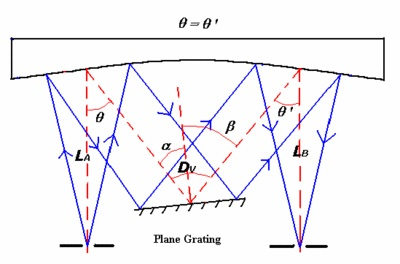
\includegraphics[width=0.7\linewidth]{Imagenes/Fastie-Ebert}}
	\subfigure[Czerny-Turnet]{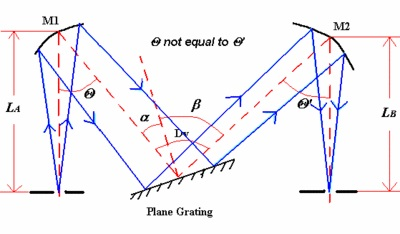
\includegraphics[width=0.7\linewidth]{Imagenes/Czerny-Turner}}
	\label{fig:Configuraciones}
	\caption[Diagramas ópticos de dos tipos de monocromadores de red de difracción.]{Diagramas ópticos de dos tipos de monocromadores de red de difracción. En la configuración (a) solo se tiene un espejo esférico, el cual se encarga de colimar y enfocar la luz, y en la configuración (b) se usan un espejo cóncavo para cada acción. Imagen tomada de. \cite{Gratings2008}} 
	
\end{figure}


\paragraph{Red de difracción.} Es el elemento dispersor del monocromador que se encarga de descomponer la luz en sus diferentes longitudes de onda, dependiendo de las dimensiones de esta así como del periodo de la red o líneas por milímetro. La red, determina el ancho del espectro que pueden trabajar.\\ 
El funcionamiento de las redes de difracción se basa en el fenómeno de difracción y de ahí su nombre. El cual ocurre cuando las ondas pasan a través de una pequeña apertura o un obstáculo perturbando así su propagación, ver figura \ref{fig:difraccion}. En la figura \ref{fig:slit2} se observa un patrón de difracción en una sola rendija.
\begin{figure}[h]
	\centering
	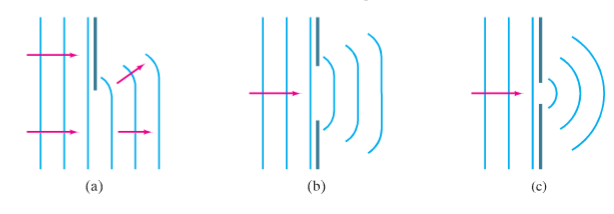
\includegraphics[width=0.9\linewidth]{Imagenes/difraccion}
	\caption{Difracción producida por un obstáculo, por un orificio grande y un orifico pequeño el cual está en el orden de la longitud de onda \cite{Oliver2013a}} %Douglas Cite
	\label{fig:difraccion}
\end{figure}
\begin{figure}[h]
	\centering
	%\subfigure[Patron de difracción ]{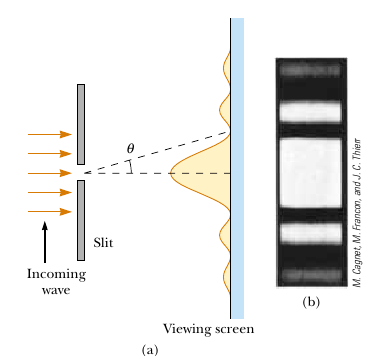
\includegraphics[width=0.48\linewidth,trim={0 10mm 0 0}]{Imagenes/2/slit1}}
	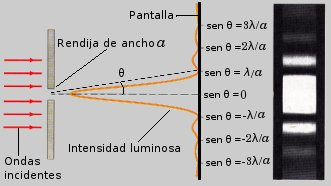
\includegraphics[width=0.7\linewidth]{Imagenes/patronrendijasimple}
	\caption{Fenómeno de difracción en una rendija. ``a'' es el ancho de la rendija. \cite{longitud01}}
	\label{fig:slit2}
\end{figure} 

En función de la longitud de onda la luz se refleja a un ángulo dado por la ecuación \ref{equa:difra2} (ver ecuación \ref{equa:difra}). Al incidir diferentes longitudes de onda se obtienen distintos valores de $\theta$ dependiendo del orden ($m$), y del ancho de la rendija $d$. 

\begin{equation}
\sin(\theta) = \frac{m \lambda}{d}
\label{equa:difra2}
\end{equation}

En la figura \ref{fig:difracro} con una longitud de onda menor se observan más ordenes que con una de mayor longitud de onda. 
El fenómeno que sucede en este proceso es el de interferencia. El cual consiste en la superposición de dos o más ondas. Se tiene la superposición constructiva y destructiva, en la primera se fortalecen las ondas y en el otro se contrarrestan. Esto se puede lograr haciendo coincidir dos o más ondas de la misma fuente en un mismo punto, cuando estas han recorrido diferentes caminos.


\begin{figure}
	\centering
	\subfigure[Laser rojo de Helio-Neón $\lambda$=632.8nm]{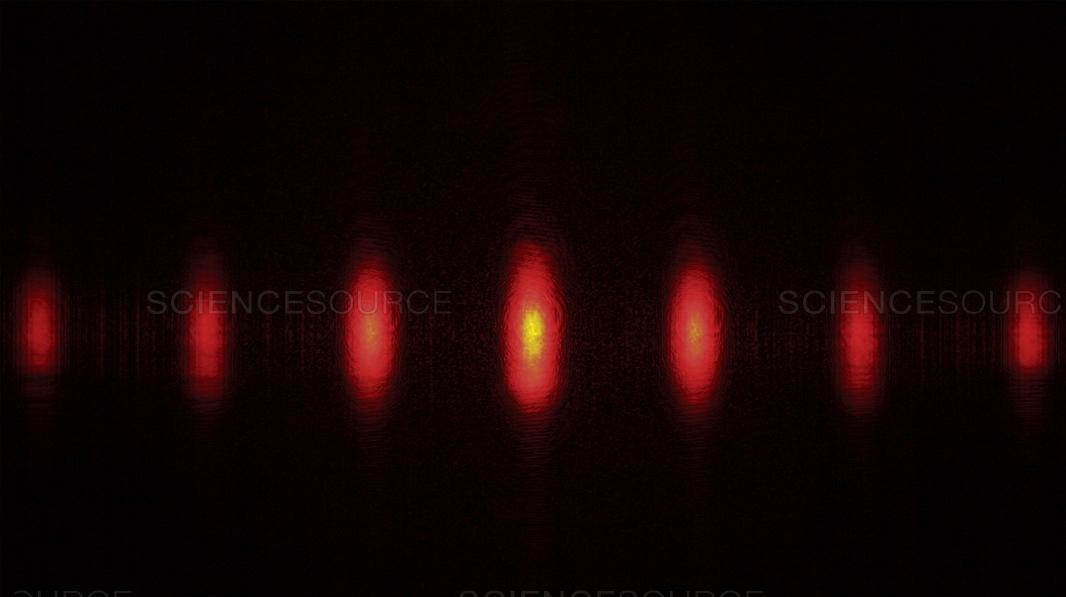
\includegraphics[width=0.48\linewidth, height=4cm]{Imagenes/2/difracRo}}
	\subfigure[Laser verde de Helio-Neón $\lambda$=543.4nm]{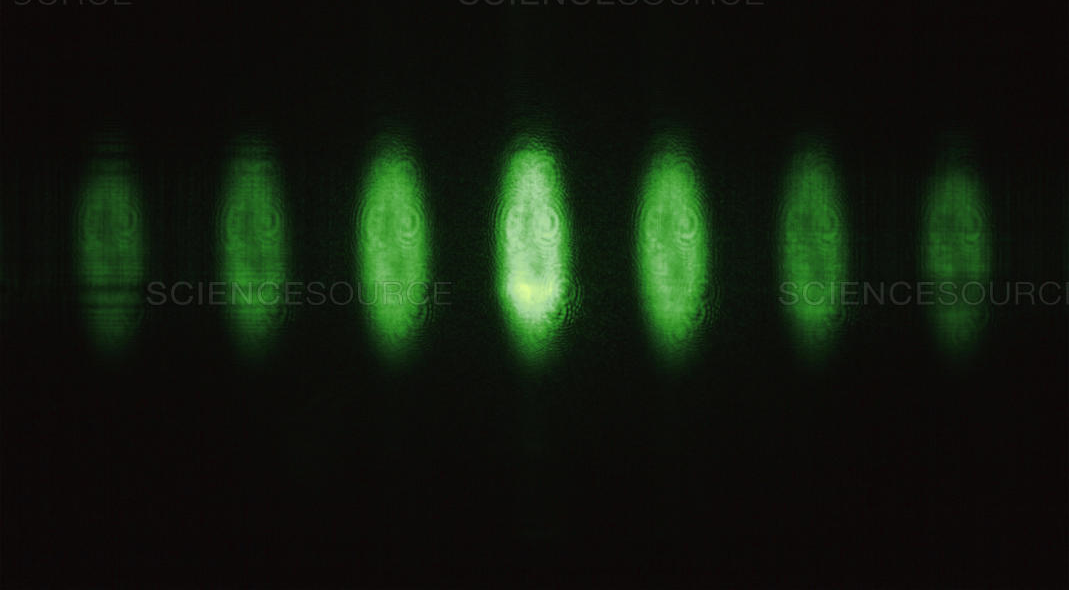
\includegraphics[width=0.48\linewidth,height=4cm]{Imagenes/2/difracGr}}
	\caption[Difracción de la luz con diferentes longitudes de onda.]{Dos láseres de Helio-Neón, rojo $\lambda$=632.8nm y verde $\lambda$=543.4nm. Son difractados en una red de 50 líneas/mm. El espacio entre cada orden de difracción es mayor en relación a la longitud de onda. \cite{laserGR}}
	\label{fig:difracro}
\end{figure}
Al momento de hacer mediciones con los espectrómetros se debe tener cuidado de no confundir los primeros órdenes de las longitudes de onda, con los demás. En la figura \ref{fig:ordenes} se ve como coinciden diferentes longitudes de onda en los mismos ángulos. Esto es de suma importancia cuando se analizan los espectros medidos, para evitar una interpretación incorrecta.

\begin{figure}[h]
	\centering
	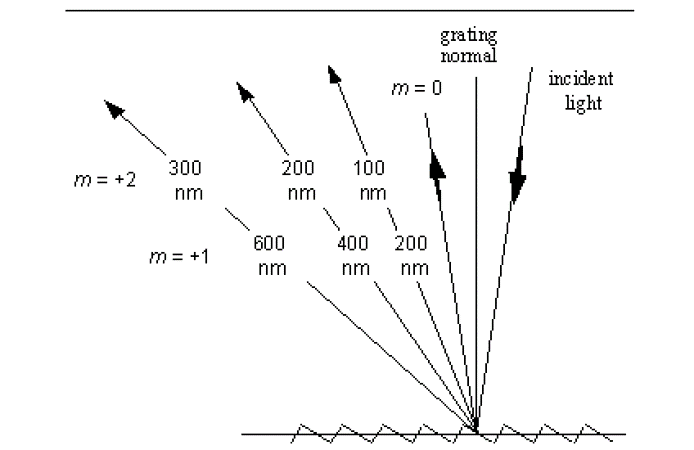
\includegraphics[width=0.7\linewidth]{Imagenes/2/ordenes}
	\caption[Difracción de la luz se aprecia el orden de difracción de diferentes longitudes de onda.]{Luz incidente es difractada y reflejada a diferentes ángulos. Se observa cómo en el mismo ángulo se encuentran dos longitudes de onda diferentes pero de diferente orden. Imagen tomada de. \cite{Palmer2005}}
	\label{fig:ordenes}
\end{figure}


%quitar esto o investigarlo bien. Texto completamente sin sentido.
La eficiencia de difracción es un valor que expresa el grado en que se puede obtener energía de la luz difractada con respecto a la luz incidida.
La eficiencia de difracción es expresada como absoluta o relativa. La primera es el porcentaje de radiación monocromática incidente que es difractada en el orden deseado. La eficiencia de difracción relativa se obtiene dividiendo la eficiencia de difracción absoluta por la reflectancia del material de recubrimiento \cite{Shimadzu}.
Las redes de difracción con alta eficiencia son deseables por muchas razones. Siendo más útiles para medir líneas de baja intensidad. \cite{Palmer2005}
% La segunda por otra parte es la relación de energía difractada en la red, comparada con un espejo recubierto del mismo material que la red

\paragraph{Poder de resolución R.} 
Es la capacidad de un espectrómetro para poder separar o resolver dos líneas espectrales contiguas. Está dado por la ecuación \ref{equa:resolucion}. Donde $\Delta\lambda$ es la diferencia entre dos longitudes de onda, m es el orden y N es la cantidad total de líneas en la red de difracción, $N= L\times W_g$, L es la longitud en milímetros de la red, y $W_g$ es la densidad de líneas por milímetro.
\begin{equation}
	R = \frac{\lambda}{\Delta \lambda}
	\label{equa:resolucion}
\end{equation}
\begin{equation}
	R = mN
	\label{equa:resolucion2}
\end{equation}

Tomemos como ejemplo una red de difracción de 1200 líneas/mm con una longitud de 110 mm, $R=mN = 1200 \times 110 = 132,000$. De la ecuación \ref{equa:resolucion}. $\Delta\lambda = \frac{R}{\lambda}$. En $\lambda_{500}$, $\Delta\lambda = 0.0038nm$
y en $\lambda_{300}$, $\Delta\lambda = 0.0022nm$. Como se ve, a menores longitudes de onda es posible distinguir entre longitudes de ondas más cercanas, y de forma inversa mientras mayor sea la longitud de onda, mayor es la distancia entre estas longitudes de onda que podrá resolver \cite{Gratings2008}.

\paragraph{Red de difracción holográfica.} Son recomendadas cuando se quiere trabajar en UV, VIS y NIR. La densidad de líneas debe ser de 1200 líneas/mm o superior. %(hasta los 6000 líneas/mm), Son muy recomendadas para trabajar en UV. 





\subsection{Motor a pasos.}
Este tipo de motores se caracterizan por tener un giro de ángulo específico, al ir cambiando la excitación de sus bobinas. %(borrado todo esto) Al tener un giro tan preciso, son utilizados en sistemas que requieran exactitud, pues el control en motores de AC o DC es más complicado debido a la inercia, así como el control de su velocidad, se desarrollaron los motores a pasos. 
Los motores a pasos se componen del estator, que es una parte fija, con cavidades, en las cuales se ubican las bobinas del motor y el rotor que es la parte móvil del motor, que va montado sobre un eje soportado por dos cojinetes lo que le permite girar libremente, ver fig. \ref{fig:rotorestator}. 

\begin{figure}[h]
	\centering
	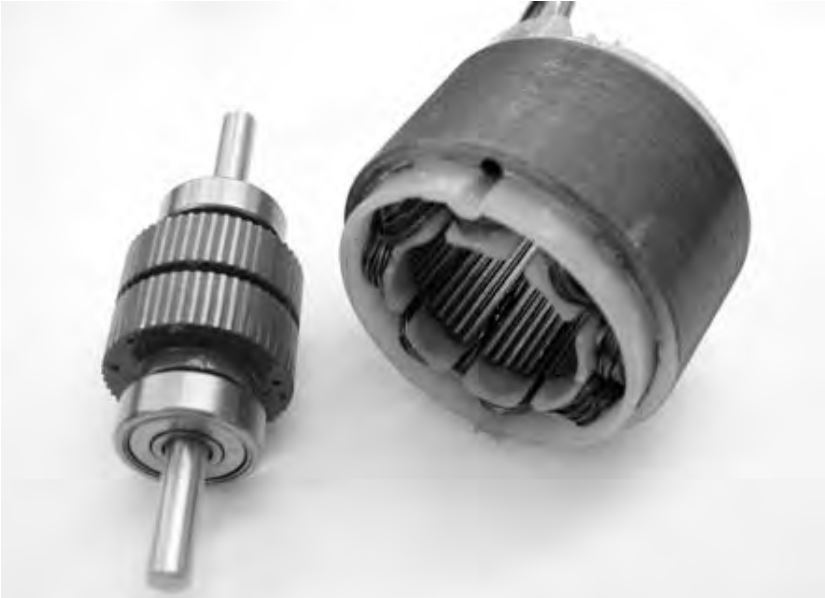
\includegraphics[width=0.7\linewidth]{Imagenes/2/RotorEstator}
	\caption{Esquema de un motor a pasos. Se observan las dos partes principales que le componen. Rotor a la izquierda y estator a la derecha. \cite{Acarnley2002}}
	\label{fig:rotorestator}
\end{figure}
El rotor del motor tiene sus polos N-S, al energizar el estator, este generará sus polos magnéticos N-S, el rotor, buscará el quedar en equilibrio magnético, Norte-Sur y Sur-Norte, lo que provoca que el rotor giré para llegar a este equilibrio. Al cambiar la excitación de las bobinas, los polos N-S creados por el estator, cambiaran, como resultado el rotor volverá a girar, para buscar el nuevo punto de equilibrio. De esta forma es como el motor va dando "pasos". En la figura \ref{fig:pasodos} para girar en el sentido de las manecillas del reloj, la bobina energizada (B), debe ser apagada, después se energiza la bobina (C), ocasionando el giro del rotor, para dar un giro desde esta posición, se deben ir encendiendo las bobinas en el siguiente orden C, D, A, B, C, desenergizando la última bobina energizada. Para girar en sentido opuesto de las manecillas del reloj simplemente se energizan las bobinas en el orden opuesto, C, B, A, D, C.
Como se aprecia, el control de un motor a pasos es realmente sencillo, y preciso. 
\begin{figure}[h!]
	\centering
	\subfigure[primer paso del motor.]{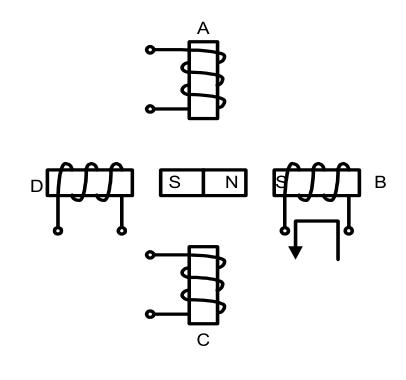
\includegraphics[width=0.4\linewidth, height = 7cm]{Imagenes/2/pasoUno}}
	\subfigure[se energiza la bobina C, y el rotor cambia de posición.]{	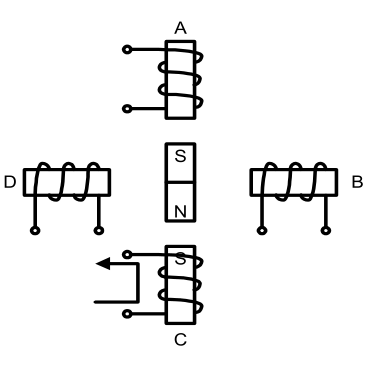
\includegraphics[width=0.4\linewidth, height = 7cm]{Imagenes/2/pasoDos}}
	\caption{Giro del rotor en sentido horario.	\cite{BasicStepper}}
	\label{fig:pasodos}
\end{figure}

Los motores a pasos se pueden clasificar en:
\begin{itemize}
	\item Motores de reluctancia variable.
	
	\item Motores de  imán permanente.
	
	\item Motores Híbridos.
	Combinan las características de los dos anteriores donde se tiene un rotor de imán permanente.
\end{itemize}


\paragraph{Control de un motor a pasos.}
El control de motores a pasos se puede realizar de diferentes formas, siguiendo simples secuencias en la alimentación de las bobinas, hay tres formas de mover el motor, paso simple, doble y medio paso. Para el paso simple se energiza solo una bobina a la vez. La secuencia se observa en la tabla \ref{tabla:pasoDobleySimple} (izquierda). Paso doble consiste en alimentar dos bobinas al mismo tiempo de tal forma que el paso se dé con más fuerza, tabla \ref{tabla:pasoDobleySimple} (derecha), pues se generan campos magnéticos en dos bobinas y no sola una. Por último el medio paso, el cual combina el paso simple y doble, logrando así que el motor deba dar el doble de pasos para recorrer la misma distancia angular, tabla \ref{tabla:medioPaso}.
%\begin{table}[]
%\centering
%\caption{Secuencia para hacer girar un motor a pasos. \cite{BasicStepper}}
%\label{tabla:SecuenciaSimple}

% \begin{tabular}{|c|c|c|c|c|c|}
%	\hline 
%	\multicolumn{6}{|c|}{Paso simple motor a pasos} \\ 
%	\hline 
%	& \hspace{5mm} A \hspace{5mm} & \hspace{5mm} B \hspace{5mm} & \hspace{5mm} C \hspace{5mm} & 	\hspace{5mm} D \hspace{5mm} & \\ 
%   \hline 
%	PASO 1  & 1 & 0 & 0 & 0 &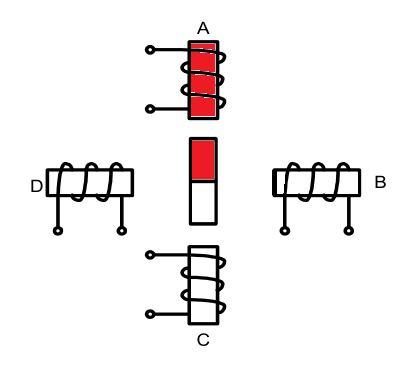
\includegraphics[width=20mm]{Imagenes/2/paso1} \\ 
%	\hline 
%	PASO 2 & 0 & 1 & 0 & 0 & 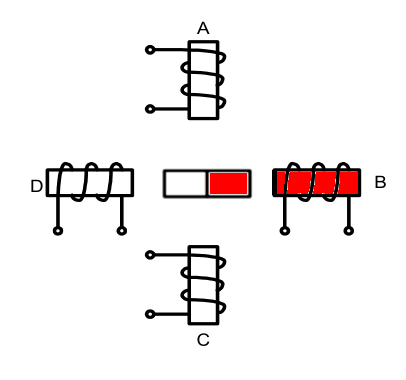
\includegraphics[width=20mm]{Imagenes/2/paso2} \\ 
%	\hline 
%	PASO 3 & 0 & 0 & 0 & 1 & 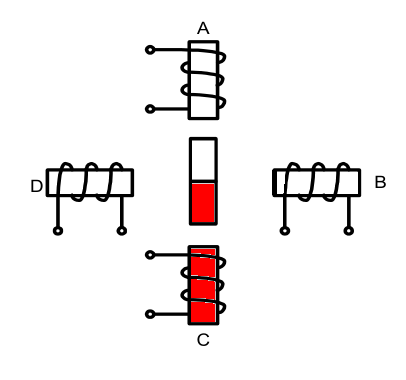
\includegraphics[width=20mm]{Imagenes/2/paso3} \\ 
%	\hline 
%	PASO 4 & 0 & 0 & 0 & 1 & 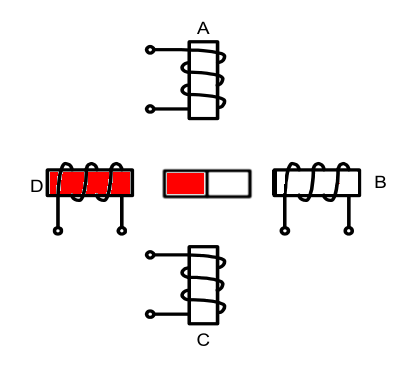
\includegraphics[width=20mm]{Imagenes/2/paso4} \\ 
%	\hline 
%\end{tabular} 
%\end{table}

\begin{table} [h!]
	\centering
	\caption[Secuencia para hacer girar un motor a pasos. \cite{BasicStepper}]{Secuencia para hacer girar un motor a pasos. Del lado izquierdo se obserba la secuencia para generar un paso simple. Del lado derecho se tiene la secuencia para un paso "doble" \cite{BasicStepper}.}
	\vspace{10mm}
	\label{tabla:pasoDobleySimple}
		\begin{tabular}{|c|c|c|c|c|c|c|c|c|c|c|c|}
			\hline 
			\multicolumn{6}{|c|}{Paso simple} & \multicolumn{6}{|c|}{Paso doble} % solución colocar 6 entre multicolumn
			\\ 
			\hline 
			 & A  &  B & C  & D & Imagen & & A & B & C & D & Imagen \\ 
			\hline 
			PASO 1  & 1 & 0 & 0 & 0 & 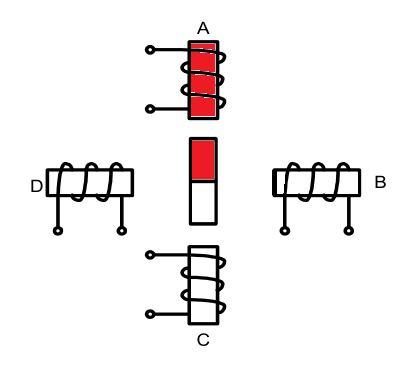
\includegraphics[width=33mm]{Imagenes/2/paso1} & PASO 1 & 1 & 1 & 0 & 0 & 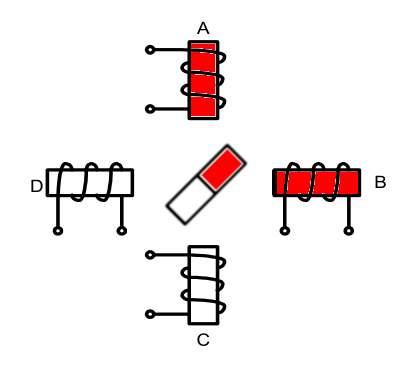
\includegraphics[width=33mm]{Imagenes/2/paso1_5}\\ 
			\hline 
			PASO 2 & 0 & 1 & 0 & 0 & 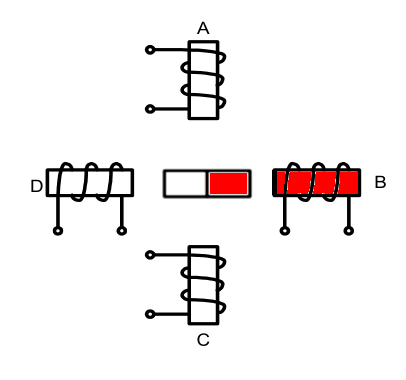
\includegraphics[width=33mm]{Imagenes/2/paso2} & PASO 2 & 0 & 1 & 1 & 0 &  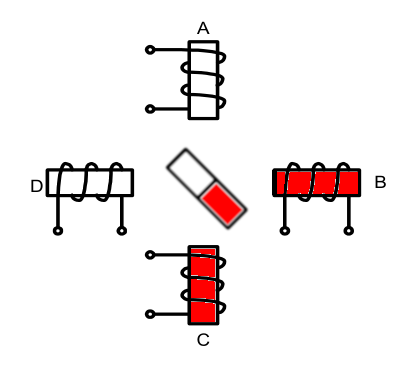
\includegraphics[width=33mm]{Imagenes/2/paso2_5} \\ 
			\hline
			PASO 3 & 0 & 0 & 1 & 0 & 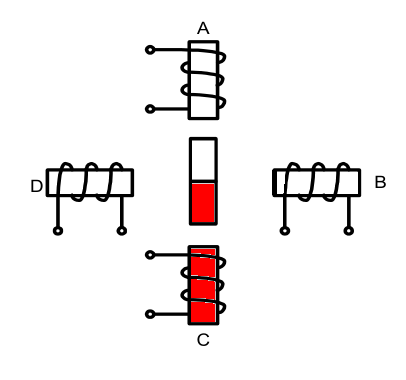
\includegraphics[width=33mm]{Imagenes/2/paso3} & PASO 3 & 0 & 0 & 1 & 1 &  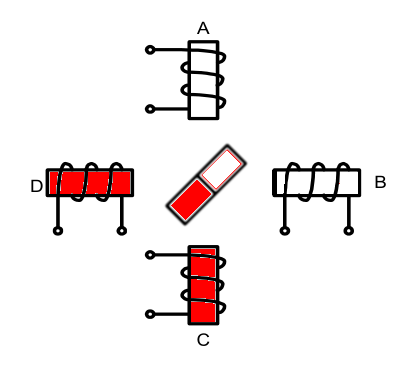
\includegraphics[width=33mm]{Imagenes/2/paso3_5} \\ 
			\hline
			PASO 4 & 0 & 0 & 0 & 1 & 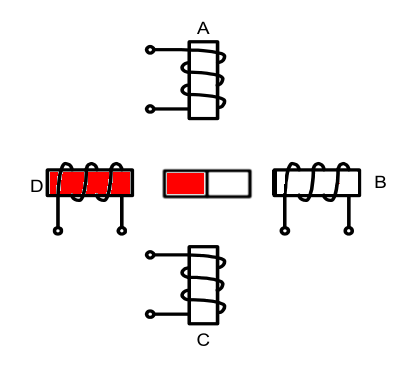
\includegraphics[width=33mm]{Imagenes/2/paso4} & PASO 4 & 1 & 0 & 0 & 1 &  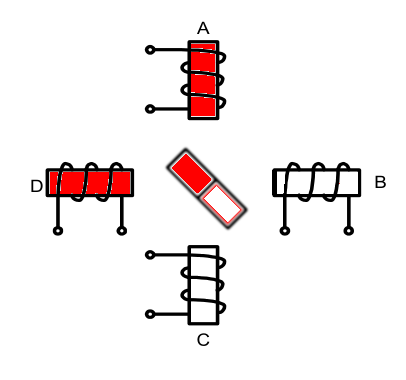
\includegraphics[width=33mm]{Imagenes/2/paso4_5} \\ 
			\hline
		\end{tabular} 
\end{table}

\begin{table}
	\centering
	\caption{Secuencia para medios pasos, se puede avanzar la mitad de un paso. \cite{BasicStepper}}
	\label{tabla:medioPaso}
	\begin{tabular}{|c|c|c|c|c|c|c|c|c|c|c|c|}
		\hline 
		\multicolumn{12}{|c|}{Medio paso} \\ 
		\hline 
		& \hspace{1mm} A \hspace{1mm} & \hspace{1mm} B \hspace{1mm} & \hspace{1mm} C \hspace{1mm} & \hspace{1mm} D \hspace{1mm} & & & \hspace{1mm} A \hspace{1mm} & \hspace{1mm} B \hspace{1mm} & \hspace{1mm} C \hspace{1mm} & \hspace{1mm} D \hspace{1mm} &  \\ 
		\hline 
		PASO 1 & 1 & 0 & 0 & 0 & 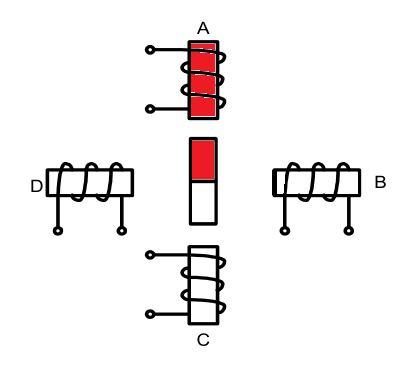
\includegraphics[width=15mm]{Imagenes/2/paso1} & PASO 5 & 0 & 0 & 1 & 0 & 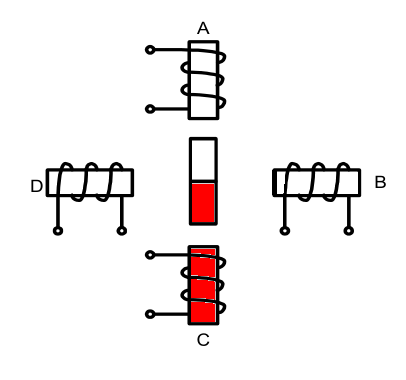
\includegraphics[width=15mm]{Imagenes/2/paso3} \\ 
		\hline 
		PASO 2 & 1 & 1 & 0 & 0 & 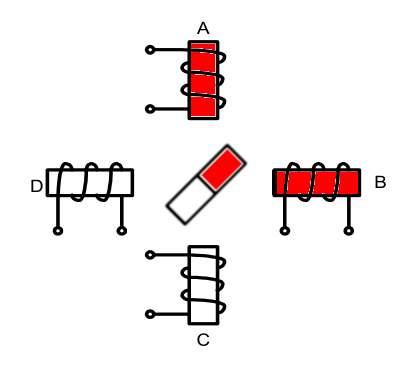
\includegraphics[width=15mm]{Imagenes/2/paso1_5} & PASO 6 & 0 & 0 & 1 & 1 & 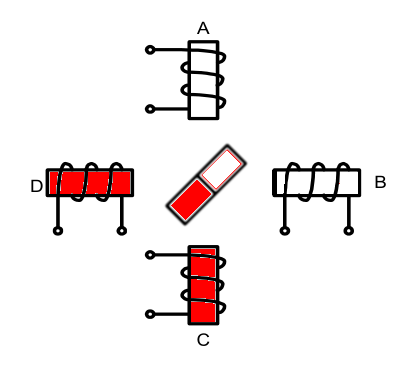
\includegraphics[width=15mm]{Imagenes/2/paso3_5} \\ 
		\hline 
		PASO 3 & 0 & 1 & 0 & 0 & 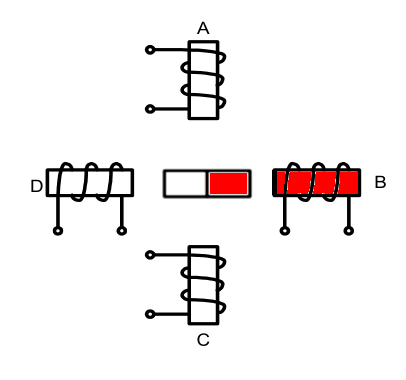
\includegraphics[width=15mm]{Imagenes/2/paso2} & PASO 7 & 0 & 0 & 0 & 1 & 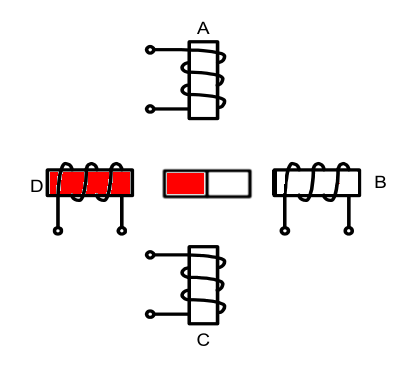
\includegraphics[width=15mm]{Imagenes/2/paso4} \\ 
		\hline 
		PASO 4 & 0 & 1 & 1 & 0 & 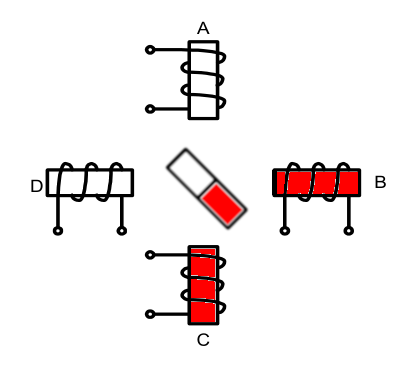
\includegraphics[width=15mm]{Imagenes/2/paso2_5} &	PASO 8  & 1 & 0 & 0 & 1 & 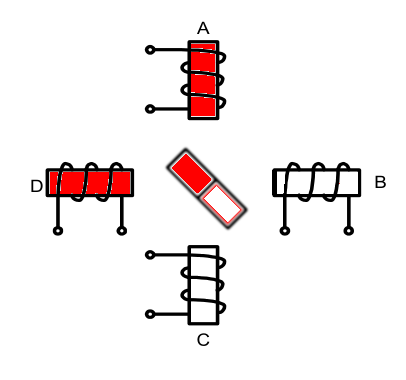
\includegraphics[width=15mm]{Imagenes/2/paso4_5} \\ 
		\hline 
	\end{tabular} 
\end{table}

Con estas secuencias y una etapa de potencia se puede controlar los motores a pasos. Para realizar estas secuencias existen circuitos integrados con 4 pines de entrada y 4 de salida, como el L293D, ver figura \ref{fig:l293}. Este contiene 2 puentes H que tienen como función el ser la etapa de potencia para el motor a pasos, dado que los microcontroladores no tienen la suficiente potencia para hacer girar el motor.
Utilizando este circuito integrado se puede hacer dos tipos de conexiones una a 4 hilos y la otra a 2 hilos. A cuatro hilos, fig. \ref{fig:bipolar-4-fils}, se pueden utilizar los tres tipos de pasos que se mencionaron antes, teniendo más opciones de control, sin embargo, el ocupar 4 pines de salida de un microcontrolador puede ser un inconveniente si es que se quiere mover más de un motor. A dos hilos, fig. \ref{fig:bipolar-2-fils}, solo se puede realizar el paso doble. %Perdemos la posibilidad de utilizar el medio paso que para ciertas aplicaciones puede ser una desventaja.

El control de los motores a pasos no es complicado, sin embargo, hoy en día existen circuitos integrados que permiten controlar los motores a pasos, lo que simplifica el trabajo para desarrollar el controlador. Entre estos circuitos integrados, \textit{drivers}, se tienen, el A4988, el DRV8825 y el TB6560, los cuales son muy comunes en las impresoras 3D, pues son de bajo costo y fáciles de cambiar. En este trabajo utilizaremos el TB6560.
\begin{figure}[h]
	\centering
	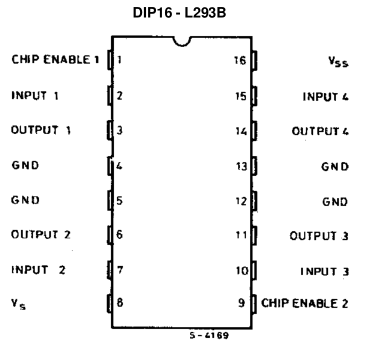
\includegraphics[width=0.4\linewidth]{Imagenes/2/L293}
	\caption[Esquema del circuito integrado L293]{Esquema del circuito integrado L293, se pueden ver los pines de entrada y salida así como el voltaje de alimentación para el circuito. \cite{L2931986}}
	\label{fig:l293}
\end{figure}

\begin{figure}[h]
	\centering
	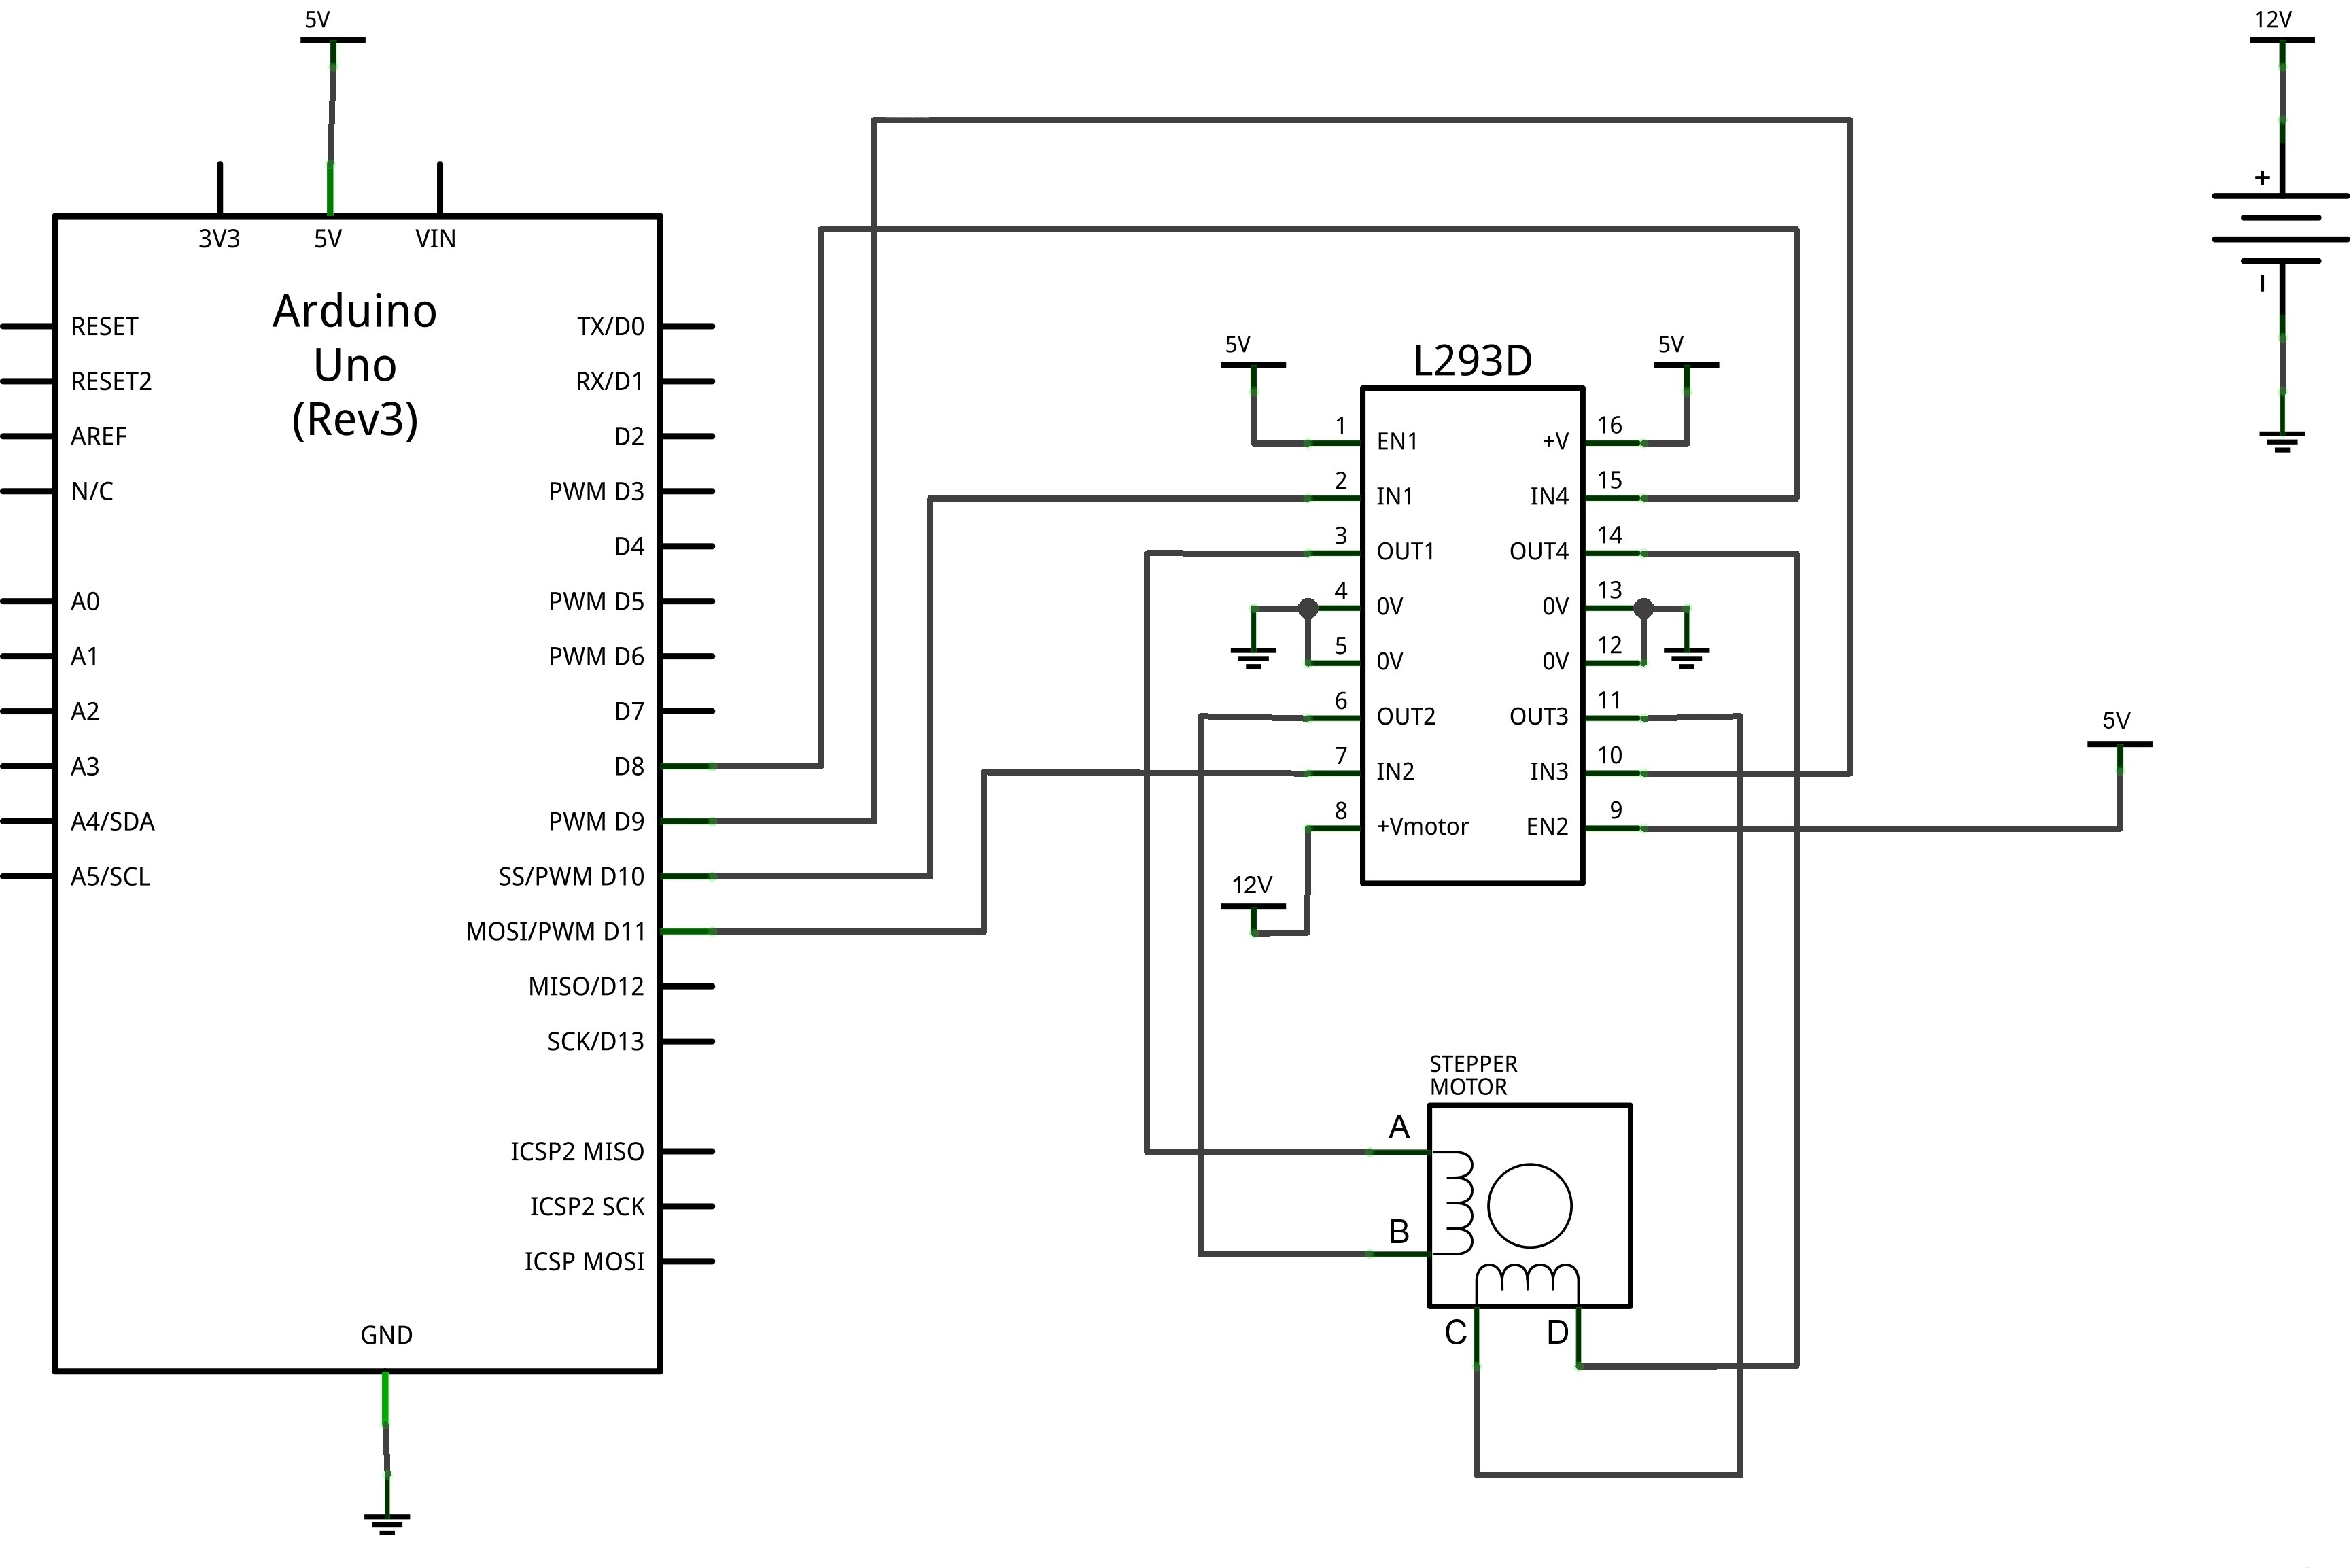
\includegraphics[width=0.7\linewidth]{Imagenes/2/BIPOLAR-4-FILS}
	\caption[Circuito para controlar el motor a pasos con un microcontrolador.]{Circuito para controlar el motor a pasos con un microcontrolador. \cite{Diymakers}}
	\label{fig:bipolar-4-fils}
\end{figure}

\begin{figure}[h]
	\centering
	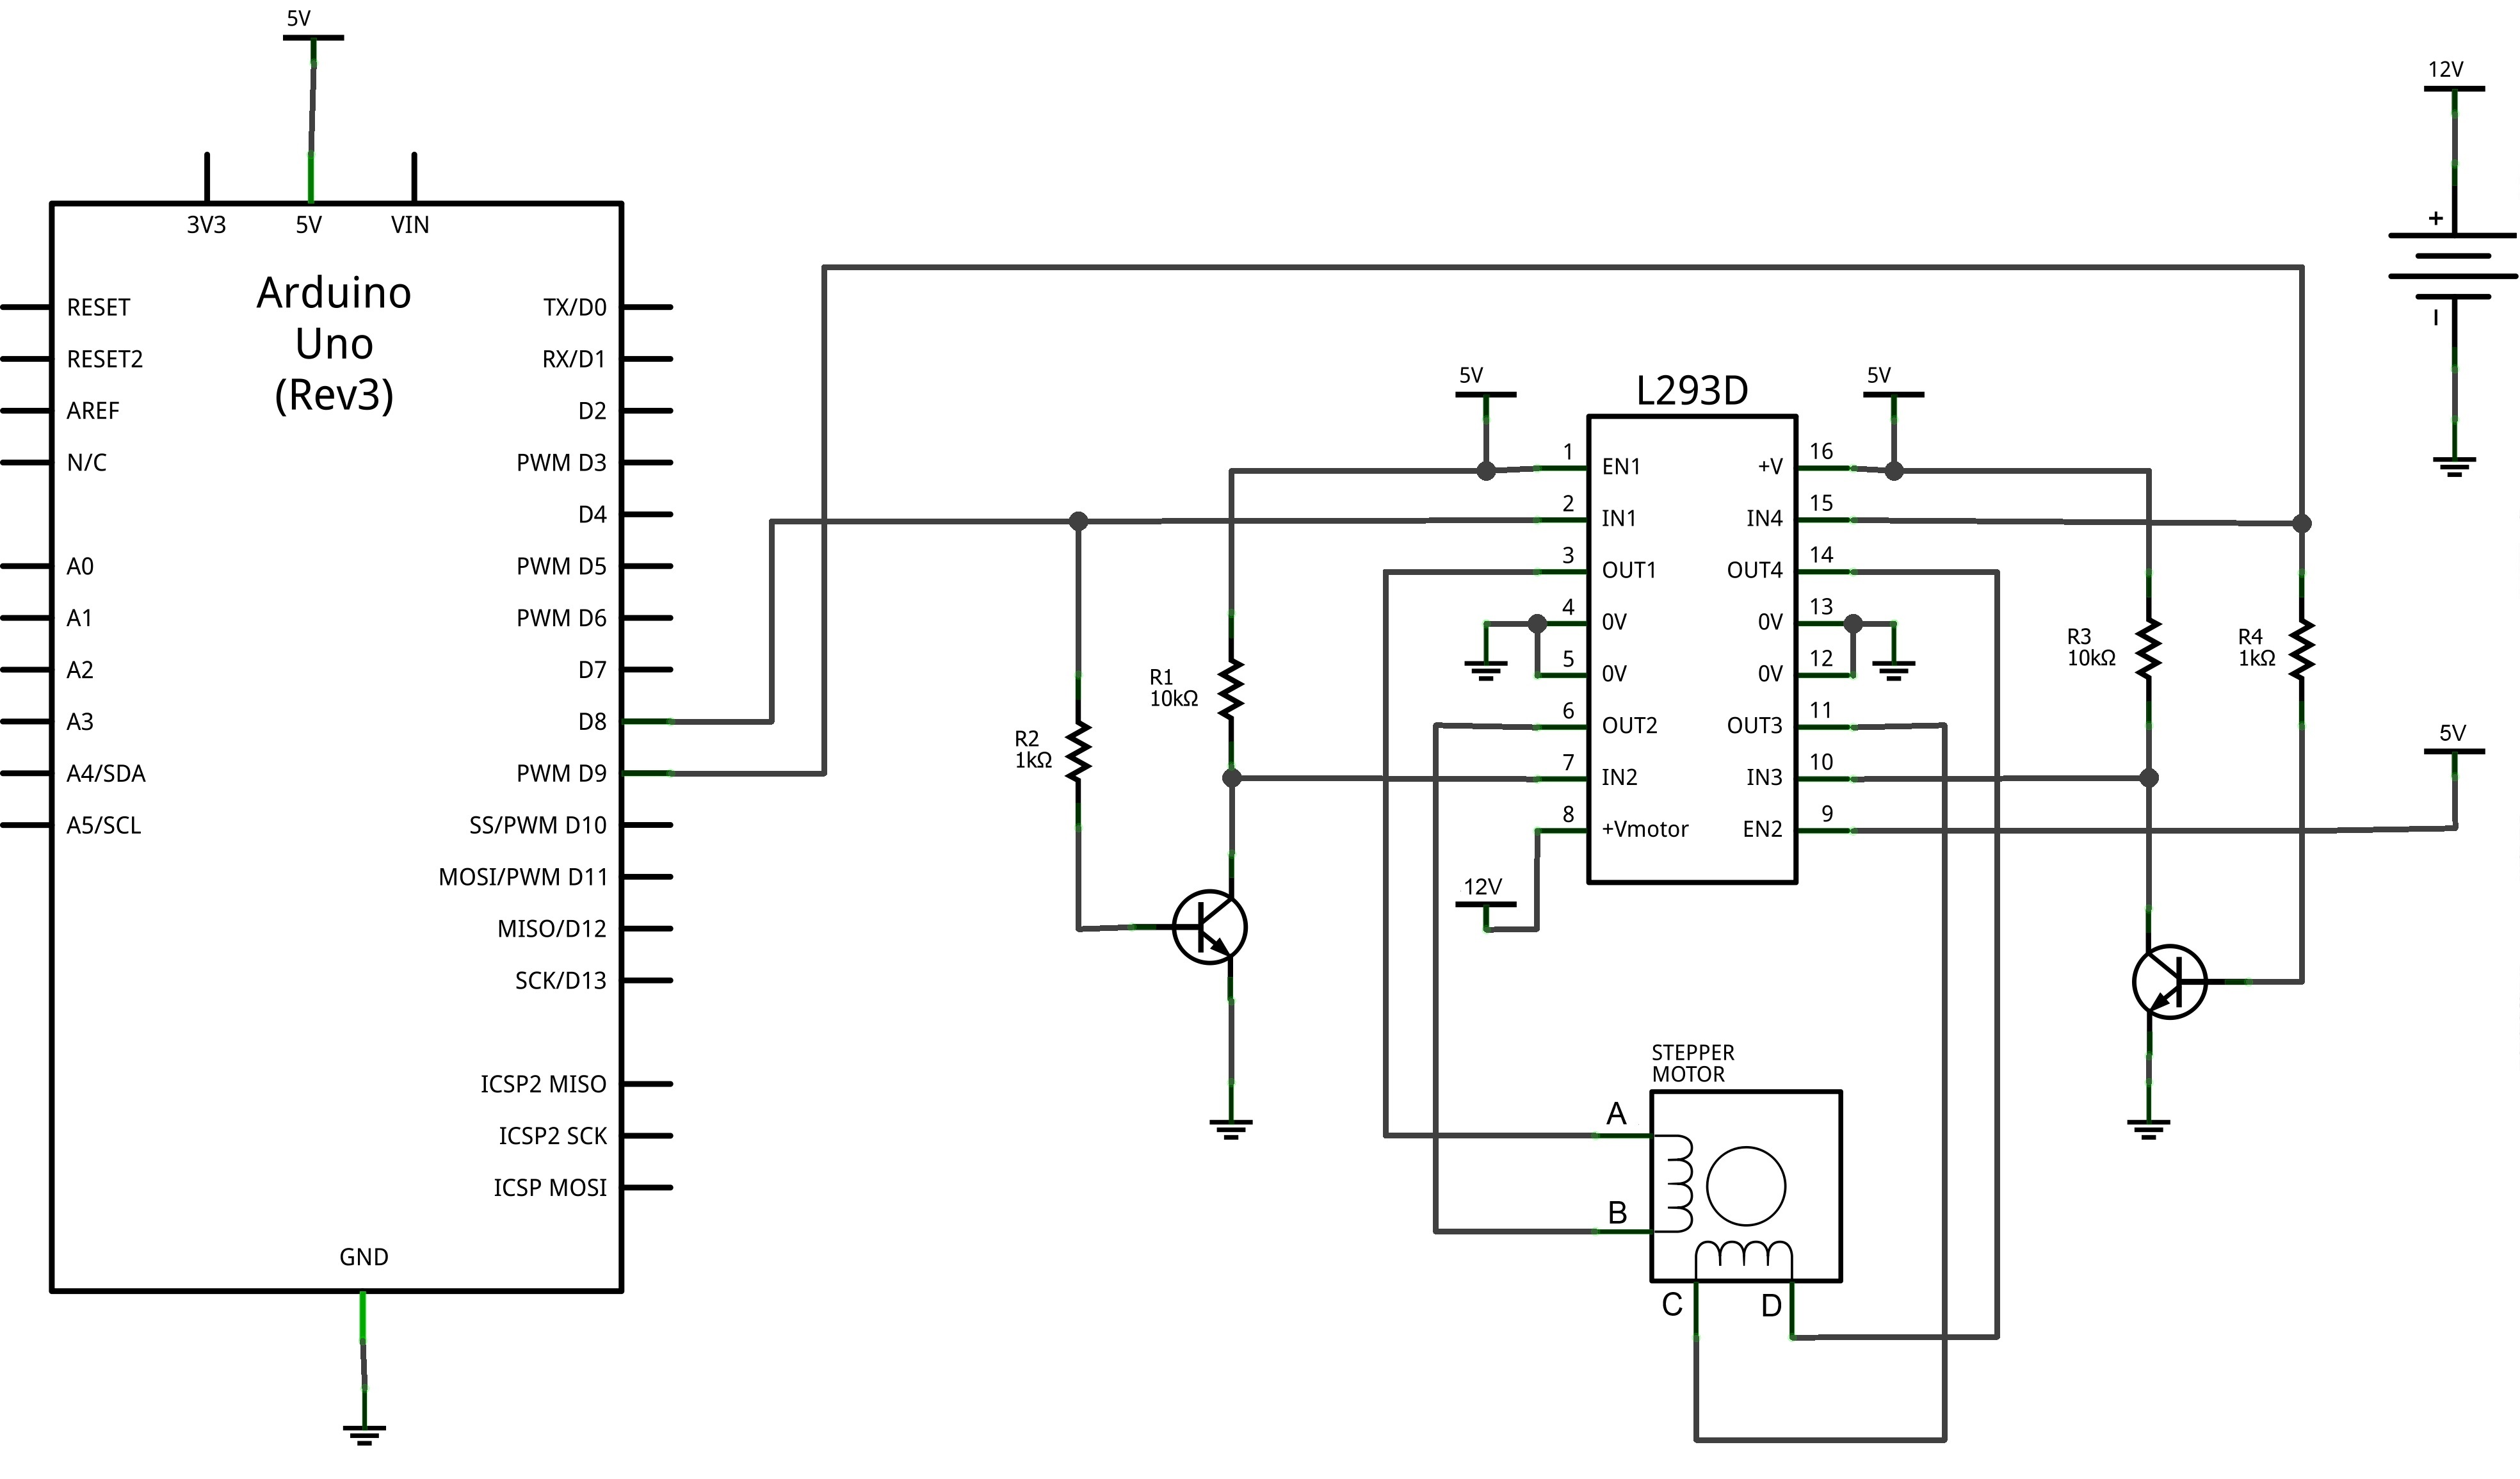
\includegraphics[width=0.8\linewidth]{Imagenes/2/bipolar-2-fils}
	\caption{Circuito utilizando solo dos pines de control. \cite{Diymakers}}
	\label{fig:bipolar-2-fils}
\end{figure}

\paragraph{Driver TB6560.}
 
Es un controlador, \textit{driver}, para motores a paso. El control de los motores a paso, se facilita con este tipo de \textit{drivers}, necesitando solo tres pines de control. Este \textit{driver}, se comercializa ya montado en una tarjeta, esta tarjeta tiene 8 entradas y 4 salidas, así como 9 \textit{switchs}. En la figura \ref{fig:tb6560}, del lado derecho se tienen tres borneras, cada una compuesta de dos pines, de abajo hacia arriba se tienen, (EN-, EN+), (CW-, CW+) y (CLK-, CLK+). Donde EN-, CW-, CLK- son GND, de entrada y las otras tres son los pines de control (EN+, CW+, CLK+), siendo controladas con valores en bajo (0V) y alto (5V, 12V y 24V máximo). A continuación, se explica su función.

\begin{itemize}
	\item EN. Es el \textit{enable}, activación del motor, si este tiene un pulso en alto (5V) el motor estará desenergizado o inhabilitado.
	\item CW. Con esta entrada se controla la dirección del motor. En bajo (0V) el motor girara en sentido horario, y en alto (5V), antihorario.
	\item CLK. Se controla la velocidad del motor, cada pulso en alto es un paso del motor.
\end{itemize}

\begin{figure}[h]
	\centering
	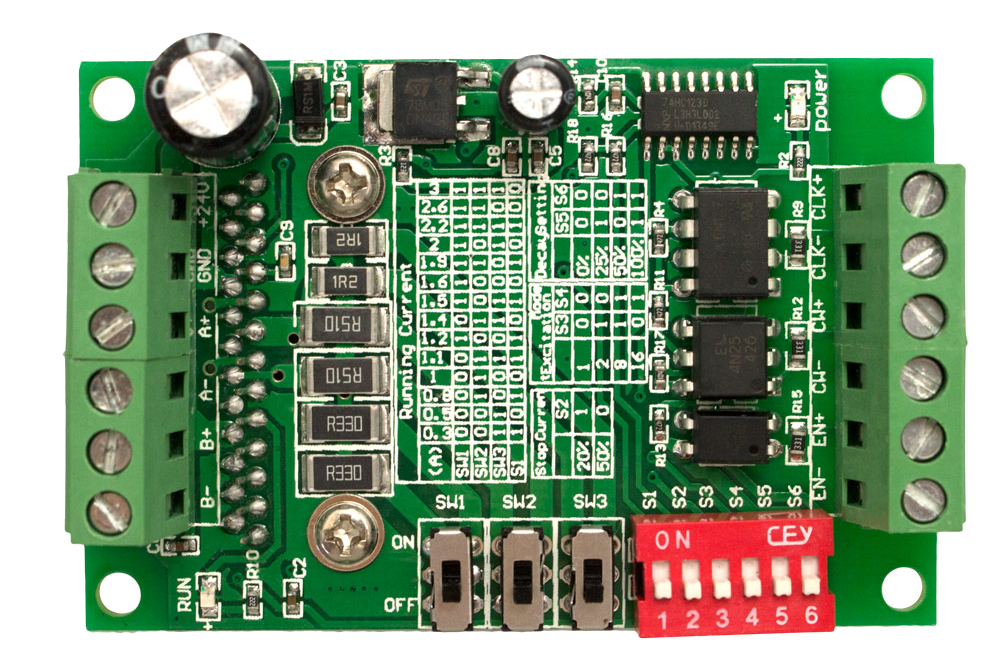
\includegraphics[width=0.7\linewidth]{Imagenes/2/TB6560a}
	\caption{Tarjeta TB6560, control para motores a pasos. \cite{TB6560}}
	\label{fig:tb6560}
\end{figure}
Del lado izquierdo se tienen otras tres borneras de dos pines cada una. De arriba hacia abajo (+24, GND, A+, A-, B+ y B-). 
\begin{itemize}
	\item +24V y GND son las entradas de voltaje para el motor a pasos, el valor máximo es 24V a 3A. 
	\item A+, A-, B+ y B-, son las salidas del \textit{driver}, conectando en estas los cables del motor a pasos, para así controlarlo.
\end{itemize} 

El driver permite limitar la corriente de operación, así como modificar el paso del motor \ref{fig:tmap0051}, logrando  $\frac{1}{16}$ de paso. Por ejemplo, un motor de 200 pasos por vuelta tiene un avance en grados de 1.8 por paso, si se utiliza la configuración de $\frac{1}{16}$ por paso, se tendrán que dar 3200 pasos por vuelta y el avance por paso será de 0.1125° por paso. Se tienen 9 \textit{switchs}:
\begin{itemize}
	\item SW1, SW2, SW3 y S1. Limitan la corriente al motor, en la figura \ref{fig:tmap0051}, en la parte superior se observa la configuración de los \textit{switchs}, para los diferentes valores de corriente.
	\item  S2. Si la corriente aumenta un $20\%$, o $50\%$ sobre el valor establecido, dependiendo de si está en alto o bajo, el motor se detendrá.
	\item  S3 y S4 sirven para variar el paso del motor como se explicó anteriormente. Pasando de paso completo a $\frac{1}{16}$
\end{itemize} 
\begin{figure}[h]
	\centering
	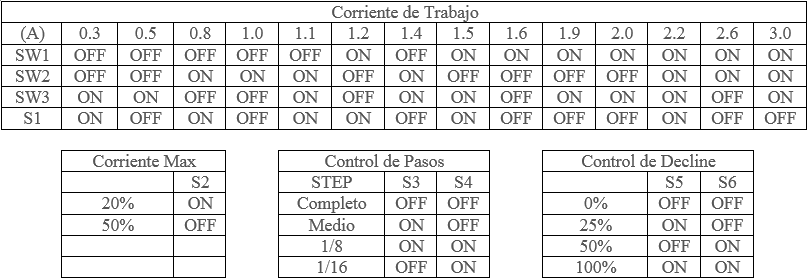
\includegraphics[width=1\linewidth]{Imagenes/2/tmap_0051}
	\caption[Configuración de la tarjeta TB6560]{Configuración de la tarjeta para corriente de trabajo y máxima, control de paso y decline. \cite{TB6560}}
	\label{fig:tmap0051}
\end{figure}

\section{Tubo fotomultiplicador.}
Los tubos fotomultiplicadores son detectores utilizados para medir potencia radiante baja, son especialmente sensibles a la radiación ultravioleta y visible, ver figura \ref{fig:pmte}. EL funcionamiento de los tubos fotomultiplicadores (PMT), se basa en el efecto fotoeléctrico.  
La luz pasa a través de la ventana, \textit{faceplate}, los fotónes inciden en el fotocátodo, y este emite electrones, a los cuales se les denomina como fotoelectrones, estos viajan por el interior del PMT.  Los fotoelectrones son acelerados con campos eléctricos y dirigidos al primer dinodo. Con lo cual se desprenden más electrones que los que incidieron, este proceso se repite en cada uno de los siguientes dinodos. Cada dinodo tiene un potencial de 100 voltios más que el anterior. Al llegar al ánodo receptor. Este proceso da como resultado que las pequeñas corrientes generadas por el fotocátodo sean amplificadas, produciendo de $10^5$ a $10^7$ electrones por cada fotón incidente.
Los tubos fotomultiplicadores, son muy sensibles, estando limitados a medir fuentes luminosas de baja potencia, de lo contrario se ocasionarían daños irreversibles en la superficie del fotocátodo.
La figura \ref{fig:pmte} es un esquemático en el que se aprecia cómo está constituido el \textit{PMT}. En la figura \ref{fig:PMT} (a) y (b) se muestran dos tubos fotomultiplicadores, la diferencia entre estos radica en donde incidirá la luz, en el (a) \textit{head-on} es en la parte frontal del \textit{PMT}, y en el (b) \textit{side-on} es el lateral. En la figura \ref{fig:pmtModule} se ven módulos de \textit{PMT}. 
 
 \begin{figure}
	\centering
	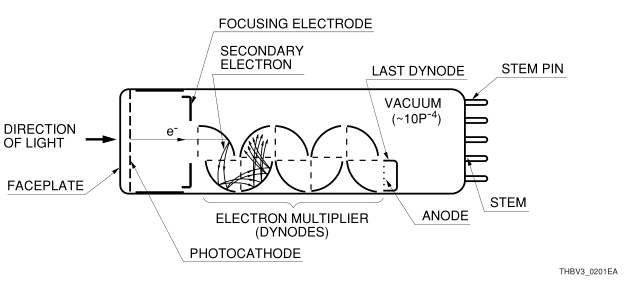
\includegraphics[width=0.9\linewidth]{Imagenes/2/PMT}
	\caption[Esquema de un tubo fotomultiplicador.]{Esquema de un tubo fotomultiplicador.\cite{Hamamatsu2006}}
	\label{fig:pmte}
\end{figure}

Los tubos fotomultiplicadores requerían de una alimentación de alto voltaje partiendo de un voltaje negativo a uno positivo. En cada uno de los dinodos del \textit{PMTs}, se tenía una diferencia de potencial de 100 volts mayor al anterior. De este modo el primer dinodo era alimentado con voltajes de $-1100$ volts hasta llegar al último dinodo el cual tenía ya un voltaje positivo menor a $100$ volts.
%posiblemente se corrija esto xD
Con los módulos de PMT ya solo se debe energizar con un voltaje de $\pm 15$ volts. Para este proyecto se va a trabajar con un módulo de tubo fotomultiplicador de la marca Hamamatsu modelo H8249.

\begin{figure}
	\centering
	\subfigure[PMT \textit{head-on}]{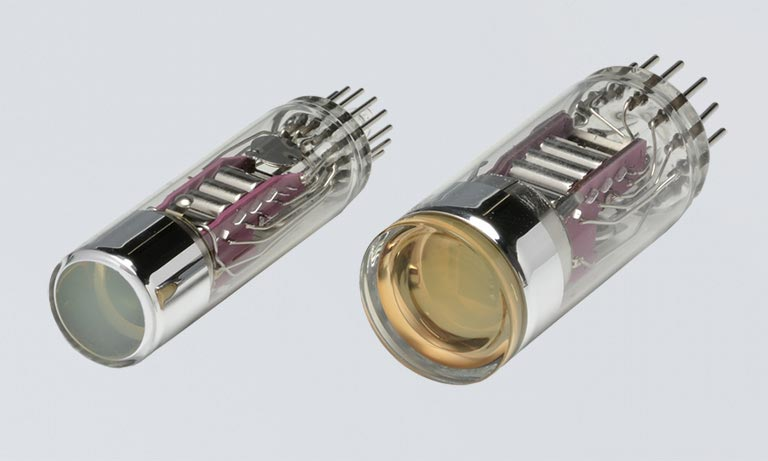
\includegraphics[width=0.4\linewidth]{Imagenes/2/PMThead}}
	\subfigure[PMT \textit{side-on}]{	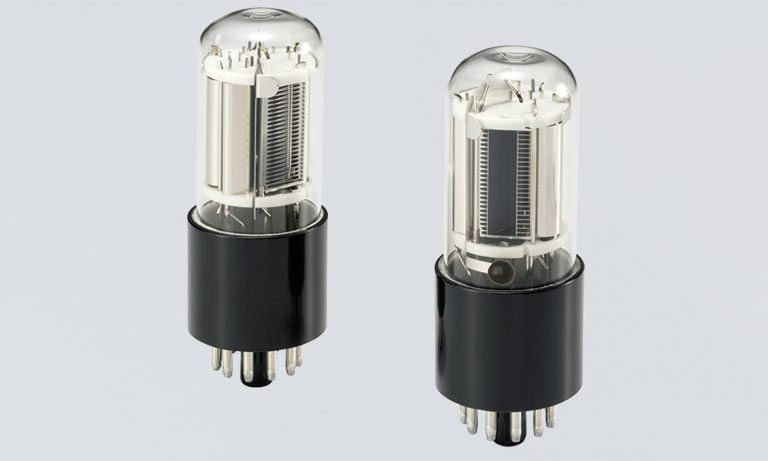
\includegraphics[width=0.4\linewidth]{Imagenes/2/PMTSide-on}}
	\caption[Tubos fotomultiplicadores]{Tubos fotomultiplicadores, de la marca Hamamatsu. \cite{Hamamatsu2007}}
	\label{fig:PMT}
\end{figure}

\begin{figure}
	\centering
	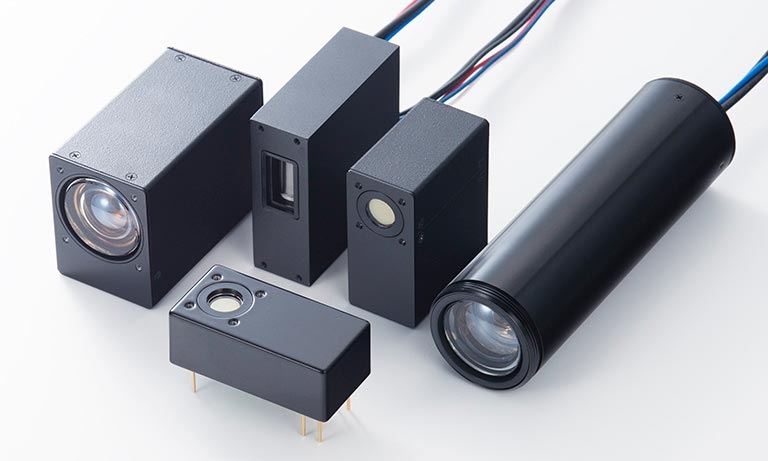
\includegraphics[width=0.7\linewidth]{Imagenes/2/PMTmodule}
	\caption{\textit{PMTs} módulos de la marca Hamamatsu. Están diseñados para diferentes aplicaciones, así como para entregar corriente o voltaje a la salida. \cite{Hamamatsu2007}}
	\label{fig:pmtModule}
\end{figure}



\paragraph{Módulo H8249-101.}
La serie H8249 incorpora un \textit{PMT-side-on}, y un circuito de fuente de alto voltaje y una amplificación de bajo ruido. El módulo entrega voltaje a la salida, en su interior cuenta con un circuito de transimpedancia con un factor de conversión de $1V/1\mu A$. El código -101 es el tipo de módulo. Su respuesta espectral va desde los $185nm$ hasta los $900nm$, cubriendo así desde el Ultravioleta medio, luz visible y parte del infrarrojo cercano.
El módulo cuenta con un ajuste de sensibilidad, figura \ref{fig:sensibilidadajuste}.

\begin{figure}[h]
	\centering
	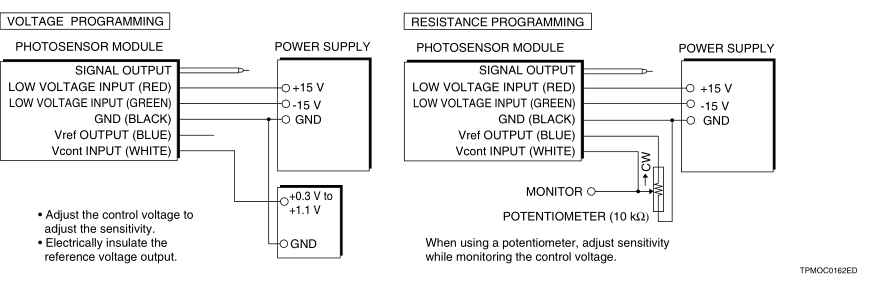
\includegraphics[width=0.8\linewidth]{Imagenes/2/SensibilidadAjuste}
	\caption[Ajuste de sensibilidad del PMT módulo H8249]{Ajuste de sensibilidad del PMT módulo H8249 puede ser controlado con una fuente de voltaje variable o utilizando una resistencia variable. Con este control se manipula la ganancia que se tendrá en el PMT. Imagen tomada de \cite{Hamamatsu2008}}
	\label{fig:sensibilidadajuste}
\end{figure}

 En la figura \ref{fig:sensibilidadajuste} se observa que el módulo se controla a través de cinco puertos o contactos, 3 de alimentación, uno de control, y el último un voltaje de referencia, que se puede usar para el control de ganancia, utilizando la configuración de resistencia programable. El voltaje del control de ganancia va desde los 0.2v hasta los 1.2v y la ganancia desde $10^{3}$ hasta $10^{7}$, ver figura \ref{fig:pmtgain}.
 \begin{figure}
 	\centering
 	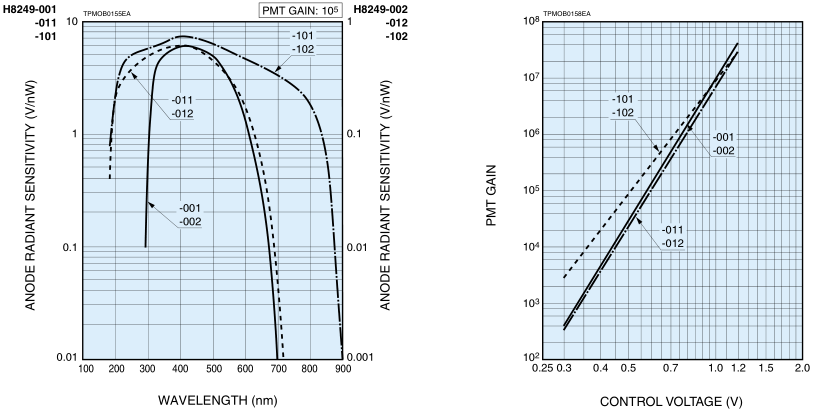
\includegraphics[width=0.7\linewidth]{Imagenes/2/PMT_GAIN}
 	\caption[Sensibilidad y ganancia H8249]{Sensibilidad del tubo fotomultiplicador (izquierda), voltaje de control apara la ganancia izquierda. Imagen tomada de. \cite{Hamamatsu2008}}
 	\label{fig:pmtgain}
 \end{figure}

\section{Microcontrolador.}
Los microcontroladores son dispositivos programables los cuales cuentan con los elementos necesarios para funcionar como una minicomputadora en un solo circuito integrado. %En el interior se encuentran: %el microprocesador, la memoria, los puertos y periféricos. Por ejemplo pensemos en un proyecto para controlar la temperatura, necesitariamos.
%\begin{itemize}
%	\item Leer la temperatura periodicamente y digitalizarla.
%	\item Un control de acuerdo a la temperatura.
%	\item mostrar la temperatura en un \textit{display} de 3 digitos.
%	\item permirir al usuario ajustar la temperatura.
%	\item Y poder configurar el sistema con una interfaz serial. 
%\end{itemize}
%Usando un microprocesador tendríamos que adquirir todas las partes por separa y armar una PCB. Figura \ref{fig:uprocesador}, Ahora que si solo usamos un microcontrolador, este ya integra varias de estos componentes en su interior, siendo más fácil su uso y su programación, figura \ref{fig:ucontrolador}. Se aprecia no solo el tamaño sino la cantidad de componentes es menor.
%Por ello es que los microcontroladores son amplimente usados en diferentes aplicaciones las cuales van desde impresoras, hornos de microondas, sistemas de adquisición de datos, controles automáticos, robots.
%\begin{figure}
%	\centering
%	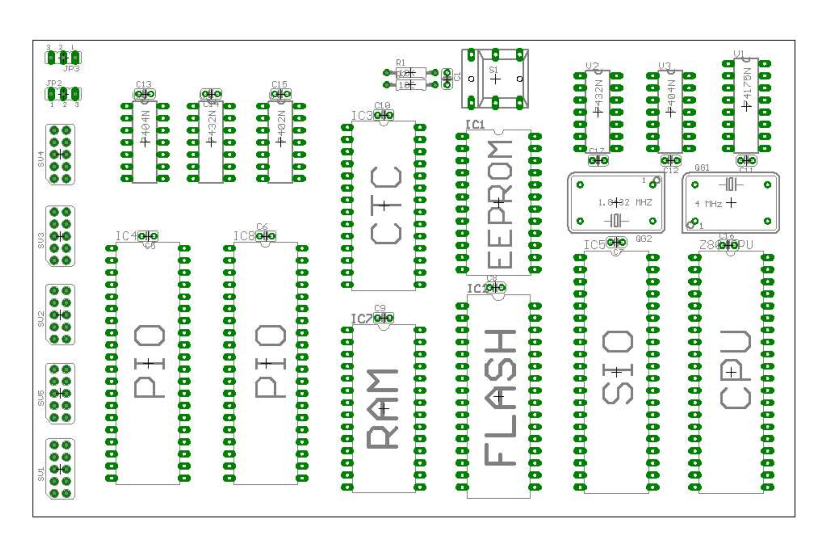
\includegraphics[width=0.7\linewidth]{Imagenes/2/uprocesador}
%	\caption{Tarjeta PCB con un procesador Z80 para 32 pines (I/O), memoria EEPROM, SRAM, \cite{Lipovski2004}}
%	\label{fig:uprocesador}
%\end{figure}
%\begin{figure}
%	\centering
%	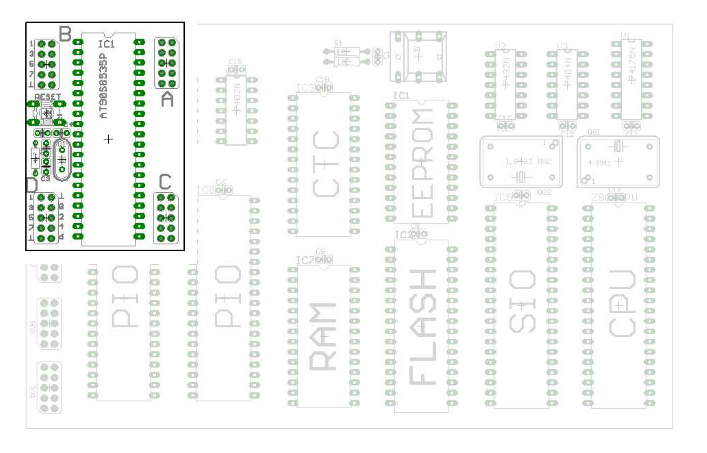
\includegraphics[width=0.7\linewidth]{Imagenes/2/ucontrolador}
%	\caption{Microcontrolador ATmega16 comparado con la tarjeta Z80}
%	\label{fig:ucontrolador}
%\end{figure}


\paragraph{Arduino.} 
Es una tarjeta que se ha popularizado en los últimos años por la facilidad de programación, así como la gran cantidad de librerías y de información en Internet. Arduino goza de una gran comunidad que día a día crean, mejoran bibliotecas y dan soporte para una gran cantidad de aplicaciones. Muchos sensores son vendidos como ``módulos'' para esta tarjeta Arduino, contando con librerías y soportes para su comunicación con softwares como MATLAB o LABVIEW. 

Programando este microcontrolador, se puede controlar y adquirir datos para el desarrollo del espectrómetro. La tarjeta Arduino Mega está basada en el microcontrolador ATmega2560, el cual cuenta con 54 pines digitales de entrada/salida, de los cuales 15 pueden ser utilizados como salidas PWM, 16 entradas analógicas, 4 UART, tiene una velocidad de 16Mhz, conexión por USB, así como una terminal ICSP. 


Para el desarrollo del sistema se requieren de.
\begin{itemize}
	\item 3 pines digitales para el control del motor a pasos.
	\item 2 pines para activar y leer un pulso de un encoder.
	\item 3 pines para el control de un potenciómetro digital.
	\item 4 pines para la comunicación SPI, para un ADC externo.
	\item 2 pines que se usan para la comunicación serial.
\end{itemize}
La tarjeta Arduino Uno, tiene los pines suficientes para este proyecto sin embargo para futuras mejoras esta tarjeta ya no serviría, por ello se decidió utilizar el Arduino Mega.

\paragraph{ADC} el ADC por sus siglas en inglés, (\textit{analog to digital converter}), es un convertidor analógico a digital. Su función es adquirir una señal eléctrica proveniente de un sensor, (voltaje o corriente) y convertirlo a una señal digital, bits. 
La resolución del ADC está dada en bits, (8, 10, 12, 16, 24 bits), o lo que es lo mismo 2 elevado a estas potencias dando como valores, (256, 1024, 4096, 65 536, 16 777 216). Mientras mayor sea el número de valores posibles del ADC menor será la diferencia en la magnitud de un bit a otro bit. Por ejemplo, teniendo un voltaje máximo de entrada de 5V para todos estos ADCs, al leer un valor de 1.2V se tendrían los valores mostrados en la siguiente tabla \ref{tabla:adcRe}.

\begin{table}[h]
\centering
\caption{Se muestra la resolución de diferentes ADCs, con un voltaje máximo de entrada de 5 volts.}
\label{tabla:adcRe}
\begin{tabular}{|c|c|c|c|}
	\hline 
	\multicolumn{4}{|c|}{Lectura de un voltaje de 1.2V} \\ 
	\hline 
	Resolución (bits) & Valor digital & voltaje leído (v) & Diferencia mínima que puede leer (mV).\\ 
	\hline 
	8  & 61.44 & 1.191 & 19.53 \\ 
	\hline 
	10 & 245.76  & 1.196 & 4.88\\ 
	\hline 
	12	& 983.04 & 1.199 & 1.22 \\ 
	\hline 
	16	& 15728.64 & 1.2 & 0.076 \\ 
	\hline 
	24	& 4026531.81 & 1.2 & 0.0003 \\ 
	\hline 
\end{tabular} 

\end{table}
\paragraph{ADC-externo.}
El ADC del Arduino Mega es de 10 bits, por lo que se buscó utilizar un ADC de mayor resolución, usando el MCP3202, ver figura \ref{fig:mcp3202}. Es un ADC de dos canales de 12 bits, con comunicación SPI, el valor máximo que puede leer es de 7 volts. El funcionamiento de los pines se explica en la tabla \ref{tabla:ADC}

\begin{figure}[h]
	\centering
	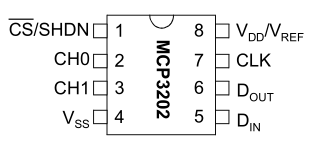
\includegraphics[width=0.5\linewidth]{Imagenes/2/MCP3202}
	\caption{ADC MCP3202 dos canales, 12 bits comunicación SPI \cite{MCP3202}}
	\label{fig:mcp3202}
\end{figure}

\begin{table}[h]
	\centering
	\caption{Tabla con las funciones de los pines del ADC MCP3202 \cite{MCP3202}}
\begin{tabular}{|c|c|}
	\hline 
	Nombre del PIN & Función  \\ 
	\hline 
	CS/SHDN & Chip select, se activa el ADC \\ 
	\hline 
	CH0 & Canal analógico 0 \\ 
	\hline 
	CH1 & Canal analógico 1 \\ 
	\hline 
	$V_{SS}$ & GND del ADC \\
	\hline
	$V_{DD}/V_{REF}$ & Alimentación y voltaje de referencia. \\  
	\hline
	CLK & Velocidad de la comunicación  \\ 
	\hline 
	$D_{IN}$ & Serial Datos de entrada \\ 
	\hline 
	$D_{OUT}$ & Serial datos salida \\ 
	\hline 

\end{tabular} 
	\label{tabla:ADC}
\end{table}

\paragraph{Potenciómetro Digital.}
Como se mencionó el \textit{PMT} necesita de un control de entrada de voltaje. Utilizando el voltaje de referencia que el propio \textit{PMT} genera se requiere un potenciómetro digital para poder variar el voltaje de control del tubo fotomultiplicador. 
El potenciómetro digital es un circuito integrado con el cual uno puede ir variando la resistencia, a través de pulsos digitales, (5v y 0v). El potenciómetro digital que se usó es el X9C103 \cite{X9C102}. El potenciómetro se observa en la figura \ref{fig:potdig}. Tiene 8 pines, su funcionamiento se explica en la tabla \ref{tabla:potpin}. %CS se activa el potenciómetro digital. Si no esta activo no se puede modificar su resistencia. INC al recibir pulsos va dando pasos en el potenciómetro digital modificando la resistencia. U/D determina si se realizará un incremento o disminución en la resistencia. $V_{CC}$ y $V_{SS}$ son la alimentación del circuito integrado, 5V y GND. $V_h/R_h$ y $V_L/R_L$ son equivalentes a las terminales de un potenciómetro mecánico. $V_W$ es la salida resultante del voltaje.
\begin{figure}[h]
	\centering
	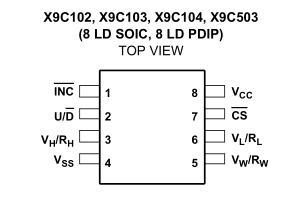
\includegraphics[width=0.5\linewidth]{Imagenes/2/potDig}
	\caption{Potenciómetro digital X9C103 \cite{X9C102}}
	\label{fig:potdig}
\end{figure}

\begin{table}[h]
	\centering
	\caption{Descripción de los pines del potenciómetro digital. \cite{X9C102} }
	\resizebox{15cm}{!}{
	\begin{tabular}{|c|c|}
		\hline 
		PIN & Descripción  \\ 
		\hline 
		INC & Incremento cada cambio de voltaje, alto a bajo, modifica la resistencia en un paso, en la dirección dada por el pin  U/D  \\ 
		\hline 
		U/D & UP/DOWN controla la dirección, (subir o bajar) la resistencia del potenciómetro. \\ 
		\hline 
		$V_H$/$R_H$ & Son los pines equivalentes a las terminales potenciómetro mecánico.  \\ 
		\hline 
		Vss & GND del potenciómetro digital. \\ 
		\hline 
		$V_W$ / $R_W$ & Es la terminal de salida del potenciómetro digital, donde veremos las variaciones de voltaje a la salida. \\ 
		\hline 
		$R_L$/ $V_L$ & Es la terminal en bajo, del potenciómetro digital. \\ 
		\hline 
		CS & el dispositivo es seleccionado cuando su entrada de voltaje está en bajo. Además se puede usar para guardar su posición. \\ 
		\hline 
		Vcc & Voltaje positivo de alimentación del potenciómetro \\ 
		\hline 
	\end{tabular} 
	}
	\label{tabla:potpin}
\end{table}

Para el PMT, se recomienda usar un potenciómetro digital de $10k\Omega$, el X9C103 es de este valor, con 100 pasos para pasar de una resistencia de 0 hasta $10k\Omega$. Esta cantidad de pasos es más que suficiente para el control de voltaje del \textit{PMT.}


\section{Interfaz gráfica.}
La interfaz gráfica, GUI,  en los sistemas es una de las partes más importante, pues es desde donde se manipula el sistema, y se observarán los datos adquiridos. Uno de los softwares más populares para hacer GUI, (del inglés \textit{Graphical User Interface}) es LabVIEW. LabVIEW es un software que ofrece un enfoque de programación gráfico, lo que lo hace más intuitivo para realizar algoritmos, analizar datos y diseñar interfaces gráficas de usuario. Es por estas características, así como la facilidad de comunicación con Arduino, que se decide utilizar este software.
LabVIEW, \textit{Laboratory Virtual Instrument Engineering Workbench} es un software desarrollado por \textit{National Instruments}. Fue desarrollado originalmente para el \textit{Apple Macintosh} en 1986. Su lenguaje gráfico es llamado "lenguaje G". Hoy en día tiene distribución para los  sistemas operativos como Windows, Unix, Linux y macOS. 








